\documentclass[a4paper,14pt,russian]{extreport}

\hoffset 0pt
\voffset 0pt

\usepackage[
  a4paper, includehead, includefoot, mag=1000,
  headsep=0mm, headheight=0mm,
  left=25mm, right=15mm, top=20mm, bottom=20mm
]{geometry}

\usepackage[T2A]{fontenc}
\usepackage[utf8]{inputenc}
\usepackage[russian]{babel}

% \usepackage{cmap} % Улучшенный поиск русских слов в полученном pdf-файле
\usepackage[unicode, pdftex]{hyperref}
\usepackage{pdfpages}
\usepackage[nottoc]{tocbibind}

\usepackage[onehalfspacing]{setspace} %"умное" расстояние между строк - установить 1.5 интервала от нормального
\usepackage{cite}  %"умные" библиографические ссылки (сортировка и сжатие)
\usepackage{indentfirst} %делать отступ в начале параграфа
\usepackage{enumerate}  %создание и автоматическая нумерация списков
\usepackage{longtable} % Длинные таблицы
\usepackage{multirow,makecell,array} % Улучшенное форматирование таблиц
\usepackage{graphicx} \graphicspath{{images/}}
\usepackage{pdflscape} % Для включения альбомных страниц
\renewcommand{\rmdefault}{ftm} % Включаем Times New Roman
%%% Выравнивание и переносы %%%
\sloppy % Избавляемся от переполнений
\clubpenalty=10000 % Запрещаем разрыв страницы после первой строки абзаца
\widowpenalty=10000 % Запрещаем разрыв страницы после последней строки абзаца
\righthyphenmin=2 % Минимальное число символов при переносе - 2.

\usepackage{fancyvrb}

\usepackage{amssymb,amsmath,amsfonts,latexsym,mathtext} %расширенные наборы  математических символов

\usepackage{amsthm}
\theoremstyle{definition}
\newtheorem{theorem}{Теорема}
\newtheorem{proposition}[theorem]{Предложение}
\newtheorem{corollary}[theorem]{Следствие}
\newtheorem{lemma}[theorem]{Лемма}
\newtheorem{definition}[theorem]{Определение}
\newtheorem{example}[theorem]{Пример}
\newtheorem{remark}[theorem]{Замечание}

\usepackage[tableposition=top]{caption}
\DeclareCaptionLabelFormat{gostfigure}{Рисунок #2}
\DeclareCaptionLabelFormat{gosttable}{Таблица #2}
\DeclareCaptionLabelSeparator{gost}{~---~}
\captionsetup{labelsep=gost}
\captionsetup[figure]{labelformat=gostfigure}
\captionsetup[table]{labelformat=gosttable}

\usepackage{fancyhdr}

\pagestyle{fancyplain}
\renewcommand{\headrulewidth}{0pt}
\fancyhf{}
\rfoot{\fancyplain{}{\thepage}}

\makeatletter 
\renewcommand\chapter{\if@openright\cleardoublepage\else\clearpage\fi \thispagestyle{fancyplain}%
\global\@topnum\z@ \@afterindentfalse \secdef\@chapter\@schapter} 
\makeatother

\addtocontents{toc}{\protect\thispagestyle{fancyplain}}

\setcounter{page}{1}

\usepackage{titlesec}
\titleformat{\chapter}
	{\normalsize\bfseries}
	{\thechapter}
	{1em}{}
	
\titleformat{\section}
	{\normalsize\bfseries}
	{\thesection}
	{1em}{}
	
\titleformat{\subsection}
	{\normalsize\bfseries}
	{\thesubsection}
	{1em}{}

\titleformat{\paragraph}
	{\normalsize\bfseries}
	{\thesection}
	{1em}{}

	
\titlespacing*{\chapter}{0pt}{-30pt}{8pt}
\titlespacing*{\section}{\parindent}{*4}{*4}
\titlespacing*{\subsection}{\parindent}{*4}{*4}
\titlespacing*{\paragraph}{\parindent}{*4}{*4}

\addto\captionsrussian{%
  \renewcommand\contentsname{CОДЕРЖАНИЕ}
  \renewcommand\appendixname{ПРИЛОЖЕНИЕ}
  \renewcommand\bibname{СПИСОК ИСПОЛЬЗОВАННЫХ ИСТОЧНИКОВ}
}

\usepackage{enumitem}
\makeatletter
    \AddEnumerateCounter{\asbuk}{\@asbuk}{м)}
\makeatother
\setlist{nolistsep}
\renewcommand{\labelitemi}{-}
\renewcommand{\labelenumi}{\asbuk{enumi})}
\renewcommand{\labelenumii}{\arabic{enumii})}

\usepackage{tocloft}
\renewcommand{\cfttoctitlefont}{\hspace{0.38\textwidth} \bfseries\MakeUppercase}
\renewcommand{\cftbeforetoctitleskip}{-1em}
\renewcommand{\cftaftertoctitle}{\mbox{}\hfill \\ \mbox{}\hfill{\footnotesize Стр.}\vspace{-2.5em}}
\renewcommand{\cftchapfont}{\normalsize\bfseries}
\renewcommand{\cftsecfont}{\hspace{31pt}}
\renewcommand{\cftsubsecfont}{\hspace{11pt}}
\renewcommand{\cftbeforechapskip}{1em}
\renewcommand{\cftparskip}{-1mm}
\renewcommand{\cftdotsep}{1}
\renewcommand{\cftchapdotsep}{\cftdotsep}
\setcounter{tocdepth}{2} % задать глубину оглавления — до subsection включительно

\newcommand{\likechapterheading}[1]{
    \newpage
    \begin{center}
    \textbf{\MakeUppercase{#1}}
    \end{center}}

\newcommand{\abbreviations}{\likechapterheading{ОБОЗНАЧЕНИЯ И СОКРАЩЕНИЯ}\addcontentsline{toc}{chapter}{ОБОЗНАЧЕНИЯ И СОКРАЩЕНИЯ}}
\newcommand{\definitions}{\likechapterheading{ОПРЕДЕЛЕНИЯ}\addcontentsline{toc}{chapter}{ОПРЕДЕЛЕНИЯ}}
\newcommand{\abbrevdef}{\likechapterheading{ОПРЕДЕЛЕНИЯ, ОБОЗНАЧЕНИЯ И СОКРАЩЕНИЯ}\addcontentsline{toc}{chapter}{ОПРЕДЕЛЕНИЯ, ОБОЗНАЧЕНИЯ И СОКРАЩЕНИЯ}}
\newcommand{\intro}{\likechapterheading{ВВЕДЕНИЕ}\addcontentsline{toc}{chapter}{ВВЕДЕНИЕ}}
\newcommand{\conclusions}{\likechapterheading{ЗАКЛЮЧЕНИЕ}\addcontentsline{toc}{chapter}{ЗАКЛЮЧЕНИЕ}}

\makeatletter
  \renewcommand{\@biblabel}[1]{#1.}	% Заменяем библиографию с квадратных скобок на точку:
\makeatother

\newcommand{\biblio}{
  \bibliographystyle{ugost2008}	% Оформляем библиографию в соответствии с ГОСТ 7.0.5
  \nocite{*}
  \bibliography{biblio}
}

\newcommand{\appendxchapter}[1]{ 
    \clearpage
    \stepcounter{chapter}    
    \chapter*{\appendixname~\Asbuk{chapter}\;#1}
    \addcontentsline{toc}{chapter}{\appendixname~\Asbuk{chapter}\;#1}
}
 

%\graphicspath{{Graphs/}{e_0/}{e_0.25/}{e_0.5/}{medium_reorientation/}{large_reorientation/}%{variant_1/}{variant_2/}{variant_3/}}

\renewcommand{\rmdefault}{cmr} % Шрифт с засечками
\renewcommand{\sfdefault}{cmss} % Шрифт без засечек
\renewcommand{\ttdefault}{cmtt} % Моноширинный шрифт

\begin{document}

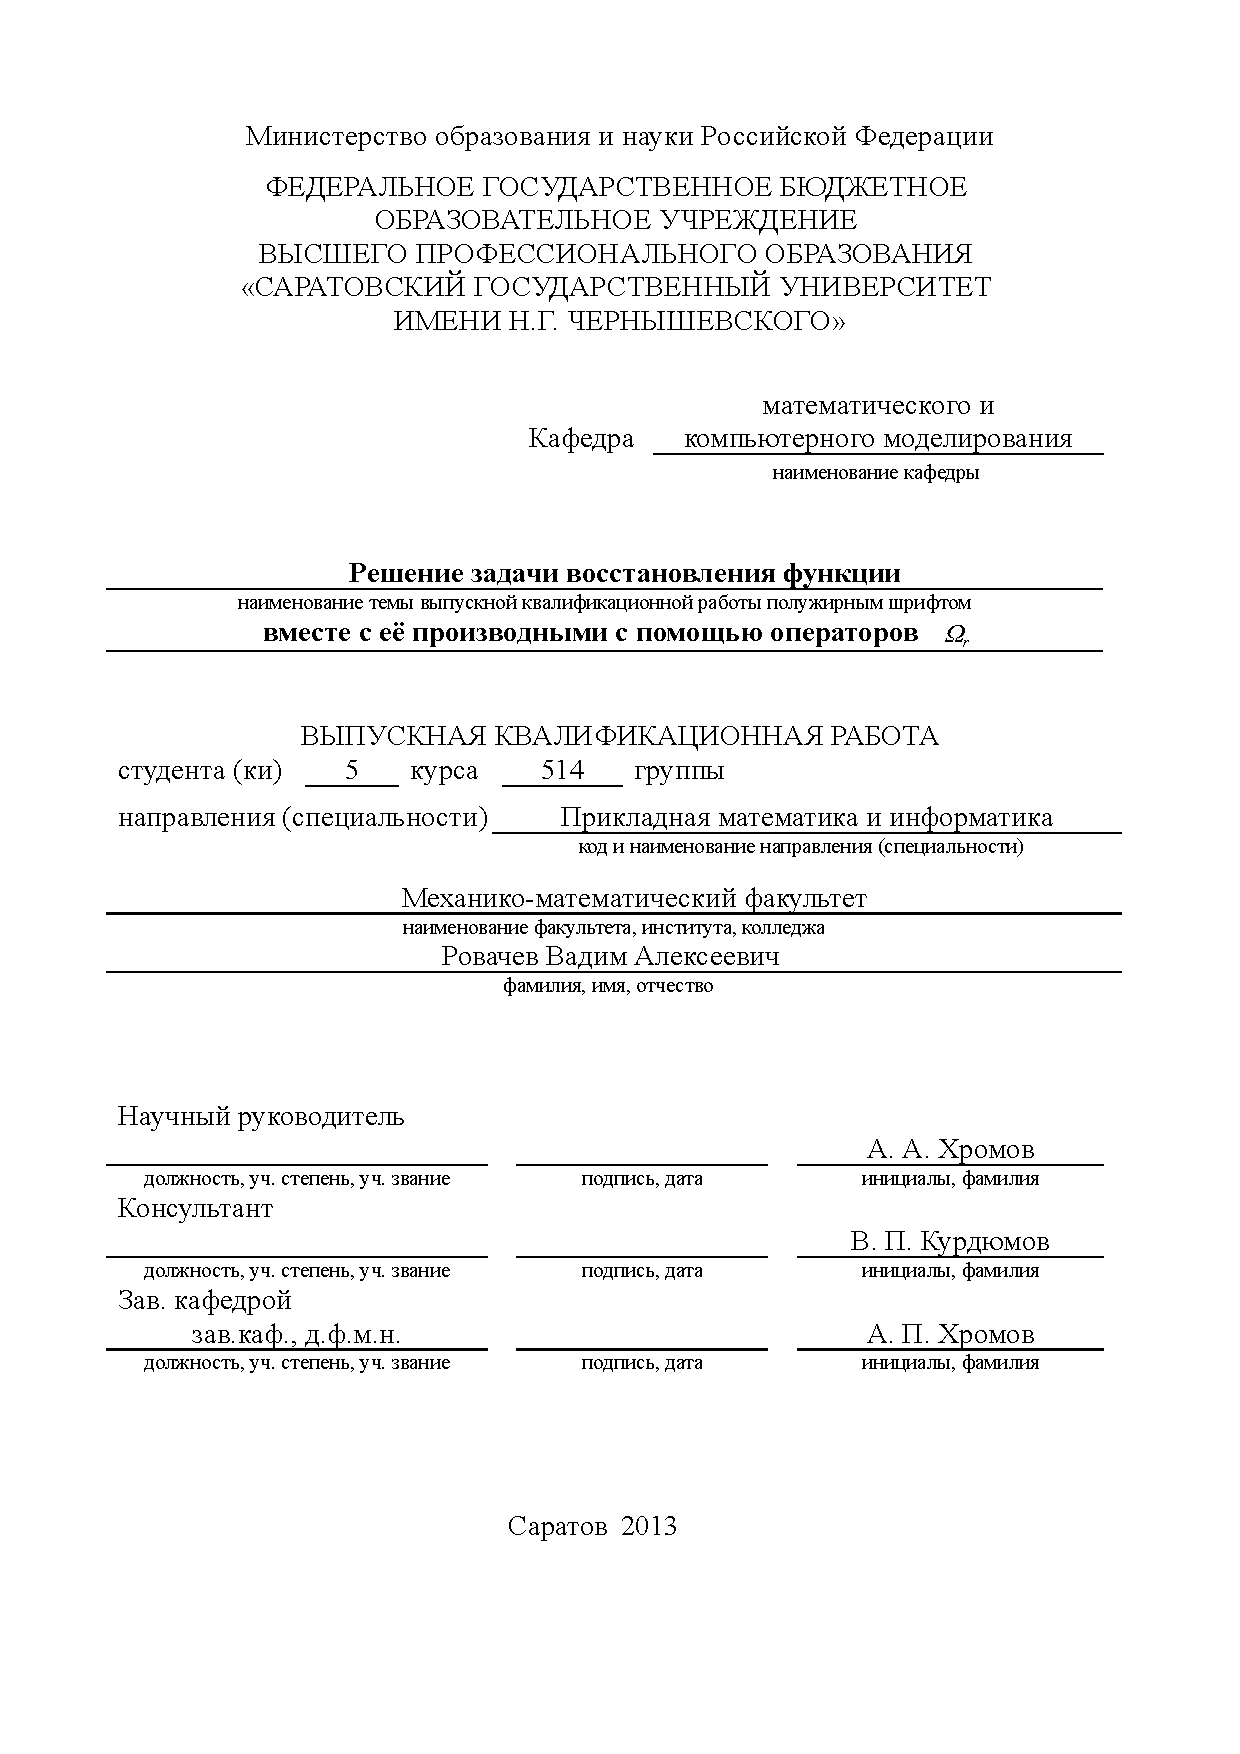
\includepdf[pages={1}]{titulDiplom.pdf}

\tableofcontents

\abbrevdef
\intro
\chapter{Приближающие свойства резольвенты оператора \\ $ L_1:y', y(0)=0 $ на отрезке $ [\varepsilon, 1] $.}
Рассмотрим простейший дифференциальный оператор первого порядка $ L_1:y^{'}, y(0)=0 $. Обозначим через $ R_\lambda(L_1) $ его резольвенту, т.е. оператор $ R_\lambda(L_1)=(L_1-\lambda E)^{-1} $, где $ E $ - единичный оператор, $ \lambda $ - спектральный параметр (числовой параметр,  вообще говоря, комплексный). Найдем формулу для резольвенты.

\section{Лемма 1.1}
\label{lemma1.1}

\textit{Для $ y(x) = R_\lambda(L_1)u$ имеет место формула:}

\begin{equation}
\begin{array}{c}

y(x) \equiv R_\lambda(L_1)u = \int\limits_0^x e^{\lambda(x-t)}u(t)dt.

\end{array}
\end{equation}

\textbf{Доказательство.} Пусть $ y = R_\lambda(L_1)u$. Тогда

\begin{equation}
\begin{array}{c}

y'- \lambda y = u,

\end{array}
\end{equation}

\begin{equation}
\begin{array}{c}

y(0)=0.

\end{array}
\end{equation}

По методу вариации произвольной постоянной общее решение уравнения (1.2) есть

\begin{equation}
\begin{array}{c}

y(x)=Ce^{\lambda x} + \int\limits_0^x e^{\lambda(x-t)}u(t)dt,

\end{array}
\end{equation}

Где $ C $ - произвольная постоянная. Находим эту постоянную из условия (1.3). Получаем $ C = 0 $. Отсюда приходим к формуле (1.1).
	
Положим в (1.1) $ \lambda \ -r $, где $ r > 0 $, и рассмотрим операторы $ rR_{-r}(L_1)$. Очевидно, эти операторы имеют вид:

\begin{equation}
\begin{array}{c}

rR_{-r}(L_1)u = r \int\limits_0^x e^{-r(x-t)}u(t)dt

\end{array}
\end{equation}

Выясним приближающие свойства операторов (1.5) при $ r \rightarrow \infty$.

\section{Лемма 1.2}
\label{lemma1.2}

\textit{Для любой функции $ u(x) \in C[0,1] $ имеет место сходимость:}

\begin{equation}
\begin{array}{c}

\Vert rR_{-r}(L_1)u-u \Vert _{C[\varepsilon ,1]} \rightarrow 0 $ \textit{при} $ r \rightarrow \infty,

\end{array}
\end{equation}

\textit{ $ \varepsilon $ - произвольное малое положительное число.}

\textbf{Доказательство.} Пусть сначала $ u(x) \in C^1[0,1] $. Тогда

\begin{equation}
\begin{array}{c}
\nonumber

\int\limits_0^x e^{-r(x-t)}u(t)dt = \frac{1}{r}\bigl\vert_0^x e^{-r(x-t)}u(t) - \frac{1}{r}\int\limits_0^x e^{-r(x-t)}u'(t)dt = \\
= \frac{1}{r} \biggl[u(x)-e^{-rx}u(0)-\int\limits_0^x e^{-r(x-t)}u'(t)dt\biggl].

\end{array}
\end{equation}

Отсюда получаем

\begin{equation}
\begin{array}{c}
\nonumber

rR_{-r}(L_1)u = u(x) - e^{-rx}u(0) - \frac{1}{r} (rR_{-r}(L_1)u').

\end{array}
\end{equation}

Тогда

\begin{equation}
\begin{array}{c}
\nonumber

rR_{-r}(L_1)u - u = u(x) - e^{-rx}u(0) - \int\limits_0^x e^{-r(x-t)}u'(t)dt.

\end{array}
\end{equation}

Далее,

\begin{equation}
\begin{array}{c}
\nonumber

\biggl| \int\limits_0^x e^{-r(x-t)}u'(t)dt \biggr| \leq \Vert u' \Vert_{C[0,1]} \int\limits_0^x e^{-r(x-t)}dt = \\
= \frac{1}{r} \Vert u' \Vert_{C[0,1]}.
(1 - e^{-rx}) 
\end{array}
\end{equation}

Тогда

\begin{equation}
\begin{array}{c}

\bigl| rR_{-r}(L_1)u - u \bigr| \leq e^{-rx} \bigl| u(0) \bigr| + \dfrac{1}{r} (1-e^{-rx})\Vert u' \Vert_{C[0,1]}.

\end{array}
\end{equation}

В силу того, что первое слагаемое в правой части последней оценки при $ x = 0 $ является константой, не зависящей от $ r $, то на всем отрезке $ [0,1] $ сходимости функций $ rR_{-r}(L_1)u $ к $ u(x) $ при $ r \rightarrow \infty $ мы отсюда не получим. Но если мы рассмотрим отрезок $ [\varepsilon, 1] $, где $ \varepsilon > 0 $ - любое фиксированное как угодно малое число, то тогда $ \Vert e^{-rx}_{C[\varepsilon,1]} = e^{-r\varepsilon} \rightarrow 0 \Vert $ при $ r \rightarrow \infty $. Отсюда следует утверждение леммы для $ u \in C^1[0,1] $.

Пусть теперь $ u(x) \in C[0,1] $. Покажем, что нормы операторов $ eR_{-r}(L_1) $, рассматриваемых как операторы из $  C[0,1] $ в $ C[\varepsilon,1] $, ограничены константой, не зависящей от $ r $.

Действительно, имеем:

\begin{equation}
\begin{array}{c}

\Vert rR_{-r}(L_1)u \Vert_{C[\varepsilon,1]} \leq \Vert rR_{-r}(L_1)u \Vert_{C[0,1]} = \\
= \Bigl\Vert r\int\limits_0^x e^{-r(x-t)}u(t)dt\Bigr\Vert_{C[0,1]} \leq \Vert u\Vert_{C[0,1]}\Vert 1 - e^{-rx}\Vert_{C[0,1]} \leq \Vert u \Vert_{C[0,1]}.

\end{array}
\end{equation}

Далее, множество функций $ u \in C^1[0,1] $ является всюду плотным в пространстве $ C[0,1] $. (Это следует из теоремы Вейерштрасса об аппроксимации непрерывной функции полиномами). Поэтому по теореме Банаха- Штейнгауза из ограниченности норм операторов $ rR_{-r}(L_1) $ отсюда следует сходимость (1.6) для любой $ u \in C[0,1] $.

Лемма доказана.

Покажем теперь, что приближающие свойства операторов $ rR_{-r}(L_1) $ сохраняются и в пространствах гладких функций, т.е. в пространствах $ C^l[0,1] $.

Пусть сначала $ u \in C^{l-1}[0,1] $. Рассмотрим операторы $ D^kR_{-r}(L_1) \equiv (R_{-r}(L_1)u)_x^{(k)} k = 1,...,l, D^1 \equiv D (Du = u')$.

\section{Лемма 1.3}
\label{lemma1.3}

\textit{Операторы $ D^kR_{-r}(L_1) $ имеют вид:}

\begin{equation}
\begin{array}{c}

D^kR_{-r}(L_1)u = u^{(k-1)}(x) - ru^{(k-2)}(x) + r^2u^{(k-3)}(x) - ... + \\
+ (-1)^{k-1}r^{k-1}u(x) + (-1)^kr^k\int\limits_0^x e^{-r(x-t)}u(t)dt, k = 1,...,l.

\end{array}
\end{equation}

\textbf{Доказательство.} Для $ k = 1 $ имеем:

\begin{equation}
\begin{array}{c}
\nonumber

DR_{-r}(L_1)u = (DR_{-r}(L_1)u)_x' = \Bigl( \int\limits_0^x e^{-r(x-t)}u(t)dt \Bigr)_x' = \\
= u(x) -r\int\limits_0^x e^{-r(x-t)}u(t)dt.

\end{array}
\end{equation}

Применяем метод математической индукции. Пусть (1.9) выполняется для $ k = m - 1 $, т.е.

\begin{equation}
\begin{array}{c}
\nonumber

D^{m-1}R_{-r}(L_1)u = u^{(m-2)}(x) - ru^{(m-3)}(x) + ... + \\
+ (-1)^{m-2}r^{m-2}u(x) + (-1)^{m-1}r^{m-1}\int\limits_0^x e^{-r(x-t)}u(t)dt.

\end{array}
\end{equation}

Тогда для $ k = m $ получим:

\begin{equation}
\begin{array}{c}
\nonumber

D^{m}R_{-r}(L_1)u = D(D^{m-1}R_{-r}(L_1)u) = u^{(m-1)}(x) - ru^{(m-2)}(x) + ... + \\
+ (-1)^{m-2}r^{m-2}u'(x) + (-1)^{m-1}r^{m-1}u(x) + (-1)^mr^m\int\limits_0^x e^{-r(x-t)}u(t)dt.

\end{array}
\end{equation}

Лемма доказана.

\section{Лемма 1.4}
\label{lemma1.4}

\textit{Если $ u(x) \in C^l[0,1] $, то имеет место сходимость:}

\begin{equation}
\begin{array}{c}

\Vert rD^k R_{-r}(L_1)u -u^{(k)}(x) \Vert_{C[\varepsilon ,1} \rightarrow 0 $ \textit{при} $ r \rightarrow \infty, k = 1,...,l.

\end{array}
\end{equation}

\textit{ $ \varepsilon $ - произвольное малое положительное число.}

\textbf{Доказательство.} Пусть $ k = 1 $. По лемме 1.3 имеем:

\begin{equation}
\begin{array}{c}

DR_{-r}(L_1)u = u(x) - r\int\limits_0^x e^{-r(x-t)}u(t)dt.

\end{array}
\end{equation}

Далее,

\begin{equation}
\begin{array}{c}

\int\limits_0^x e^{-r(x-t)}u(t)dt = e^{-rx}\int\limits_0^x e^{rt}u(t)dt = \\
= e^{-rx} \big\vert_0^x \frac{1}{r} e^{rt}u(t) - \frac{1}{r}\int\limits_0^x e^{-r(x-t)}u'(t)dt = \\
= \frac{1}{r}u(x) - \frac{1}{r} e^{-rx}u(0) - \frac{1}{r}\int\limits_0^x e^{-r(x-t)}u'(t)dt

\end{array}
\end{equation}

Подставляя (1.12) в (1.11), получим:

\begin{equation}
\begin{array}{c}
\nonumber

DR_{-r}(L_1)u = e^{-rx}u(0) + \int\limits_0^x e^{-r(x-t)}u'(t)dt

\end{array}
\end{equation}

или

\begin{equation}
\begin{array}{c}

DR_{-r}(L_1)u = R_{-r}(L_1)u' + e^{-rx}u(0).

\end{array}
\end{equation}

Получим аналогичное (1.13) выражение для $ D^kR_{-r}(L_1) $ при $ k > 1 $. 

В силу (1.13) имеем:

\begin{equation}
\begin{array}{c}
\nonumber

D^2R_{-r}(L_1)u = D(DR_{-r}(L_1)u) = D[R_{-r}(L_1)u' + e^{-rx}u(0)] = \\
= DR_{-r}(L_1)u' - re^{-rx}u(0).

\end{array}
\end{equation}

Опять применяем (1.13), заменив $ u $ на $ u' $.

Получаем:

\begin{equation}
\begin{array}{c}
\nonumber

D^2R_{-r}(L_1)u = R_{-r}(L_1)u'' + e^{-rx}u'(0) - re^{-rx}u(0).

\end{array}
\end{equation}

Покажем, что в общем случае для любого $ k $ справедлива формула:

\begin{equation}
\begin{array}{c}

D^kR_{-r}(L_1)u = R_{-r}(L_1)u^{(k)} + e^{-rx}u^{(k-1)}(0) -er^{-rx}u^{(k-2)}(0) + ... + \\
+ (-1)^{k-1}r^{k-1}e^{-rx}u(0).

\end{array}
\end{equation}

Мы показали, что (1.14) выполняется для $ k = 1,2 $. Пусть это соотношение выполняется для $ k = m - 1 $, т.е.

\begin{equation}
\begin{array}{c}
\nonumber

D^{m-1}R_{-r}(L_1)u = R_{-r}(L_1)u^{(m-1)} + e^{-rx}u^{(m-2)}(0) - re^{-rx}u^{(m-3)}(0) + ... + \\
+ (-1)^{m-2}r^{m-2}e^{-rx}u(0).

\end{array}
\end{equation}

Тогда

\begin{equation}
\begin{array}{c}
\nonumber

D^mR_{-r}(L_1)u = D(D^{m-1}R_{-r}(L_1)u) = DR_{-r}(L_1)u^{(m-1)} + \\
+ D\bigl[e^{-rx}u^{(m-2)}(0) - re^{-rx}u^{(m-3)}(0) + ... + (-1)^{m-2}r^{m-2}e^{-rx}u(0)\bigr].

\end{array}
\end{equation}

Используя (1.13) с заменой $ u(x) $ на $ u^{(m-1)}(x) $, придём к выражению:

\begin{equation}
\begin{array}{c}
\nonumber

D^mR_{-r}(L_1)u = R_{-r}(L_1)u^{(m)} + e^{-rx}u^{(m-1)}(0) - re^{-rx}u^{(m-2)}(0) + \\
+ r^2e^{-rx}u^{(m-3)}(0) + ... + (-1)^{m-1}r^{m-1}e^{-rx}u(0).

\end{array}
\end{equation}

Из формулы (1.14) получаем оценку:

\begin{equation}
\begin{array}{c}
\nonumber

\bigl\Vert rD^kR_{-r}(L_1)u - u^{(k)}\bigr\Vert_{C[\varepsilon ,1]} \leq \bigl\Vert rR_{-r}(L_1)u^{(k)} - u^{(k)}\bigr\Vert_{C[\varepsilon ,1]} + e^{-r\varepsilon}\sum\limits_{j=0}^{k-1} r^j\vert u^{(k-j-1)}(0)\vert,

\end{array}
\end{equation}

И тогда соотношение (1.10) вытекает из леммы 1.2.

\textbf{Замечание}. Если в лемме 1.2 $ u(0) = 0 $, то сходимость (1.6) будет выполняться при $ \varepsilon = 0$, т.е. на всем отрезке $ [0,1] $. Если в лемме 1.4 $ u^{(m)}(0) = 0, m = 0,1,...,k $, , то сходимость 1.10 будет выполняться также при $ \varepsilon = 0 $.

В дальнейшем нам потребуются свойства не только самих операторов $ rR_{-r}(L_1) $, но и их степеней – операторов $ (rR_{-r}(L_1))^k $.

\section{Лемма 1.5}
\label{lemma1.5}

\textit{Операторы $ (rR_{-r}(L_1))^k $ имеют вид:}

\begin{equation}
\begin{array}{c}

(rR_{-r}(L_1))^ku = r^k\int\limits_0^x \dfrac{(x-t)^{k-1}}{(k-1)!}e^{-r(x-t)}u(t)dt.

\end{array}
\end{equation}

\textbf{Доказательство.} Обозначим для краткости $ rR_{-r}(L_1) = \Omega_{1r} $. Тогда для $ k = 2 $ имеем:

\begin{equation}
\begin{array}{c}
\nonumber

\Omega_{1r}^2u = r^2\int\limits_0^x e^{-r(x-t)} \int\limits_0^t e^{-r(x-t)} u(\tau)d\tau dt = \\
= r^2e^{-rx}\int\limits_0^x\int\limits_0^t e^{r\tau}u(\tau)d\tau dt = r^2e^{-rx}\int\limits_0^x\int\limits_\tau^x dte^{r\tau}u(\tau)d\tau = \\
= r^2e^{-rx}\int\limits_0^x (x-\tau)e^{r\tau}u(\tau)d\tau = r^2\int\limits_0^x (x-\tau)e^{-r(x-t)}u(\tau)d\tau .

\end{array}
\end{equation}

Заменим обозначение $ \tau $ на $ t $, получим (1.15) при $ k = 2 $. 

Пусть для $ k = m - 1 $ выполняется формула (1.15), т.е.

\begin{equation}
\begin{array}{c}
\nonumber

\Omega_{1r}^{m-1}u = r^{m-1}\int\limits_0^x\dfrac{(x-t)^{m-2}}{(m-2)!}e^{-r(x-t)}u(t)dt.

\end{array}
\end{equation}

Тогда

\begin{equation}
\begin{array}{c}
\nonumber

\Omega_{1r}^mu = \Omega_{1r}(\Omega_{1r}^{m-1}u) = r^m\int\limits_0^x e^{-r(x-t)} \int\limits_0^t\dfrac{(t-\tau)^{m-2}}{(m-2)!}e^{-r(t-\tau)}u(\tau)d\tau dt = \\
= r^me^{-rx}\int\limits_0^x\int\limits_0^t\dfrac{(t-\tau)^{m-2}}{(m-2)!}e^{r\tau}u(\tau)d\tau dt = \\
= r^me^{-rx}\int\limits_0^x\int\limits_\tau^x\dfrac{(t-\tau)^{m-2}}{(m-2)!}dte^{r\tau}u(\tau)d\tau = \\
= r^m\int\limits_0^x\dfrac{(x-\tau)^{m-1}}{(m-1)!}e^{-r(x-t)}u(\tau)d\tau,

\end{array}
\end{equation}

что и требовалось доказать.

\section{Лемма 1.6}
\label{lemma1.6}

\textit{Если $ u \in C^1[0,1] $, то операторы $ \Omega_{1r}^k $ имеют представление:}

\begin{equation}
\begin{array}{c}

\Omega_{1r}^ku = -\dfrac{r^{k-1}x^{k-1}e^{-rx}}{(k-1)!}u(0) + \Omega_{1r}^{k-1}u - \dfrac{1}{r}\Omega_{1r}^ku',

\end{array}
\end{equation}

\textit{где $ k \geq 2 $.}

\textbf{Доказательство.} Пусть $ k = 2 $.  Тогда из (1.15) мы получаем:

\begin{equation}
\begin{array}{c}
\nonumber

\Omega_{1r}^2u = r^2\int\limits_0^x (x-t)e^{-r(x-t)}u(t)dt.

\end{array}
\end{equation}
Интегрируем по частям:
\begin{equation}
\begin{array}{c}
\nonumber

\Omega_{1r}^2u = r^2\biggl\lbrace \dfrac{1}{r} \Big\vert_0^x e^{-r(x-t)}(x-t)u(t) - \dfrac{1}{r} \int\limits_0^x e^{-r(x-t)}[-u(t) + (x - t)u'(t)]dt \biggr\rbrace = \\
= r \biggl[ -xe^{-rx}u(0) + \int\limits_0^x e^{-r(x-t)}u(t)dt - \int\limits_0^x e^{-r(x-t)}(x-t)u'(t)dt \biggr] = \\
= -rxe^{-rx}u(0) + \Omega_{1r}u - \dfrac{1}{r}\Omega_{1r}^2u'.

\end{array}
\end{equation}

Предположим, что (1.16) выполняется для $ k = m - 1, m > 2 $. Тогда

\begin{equation}
\begin{array}{c}
\nonumber

\Omega_{1r}^{m-1}u = -\dfrac{r^{m-2}x^{m-2}e^{-rx}}{(m-2)!}u(0) + \Omega_{1r}^{m-2}u - \dfrac{1}{r}\Omega_{1r}^{m-1}u.

\end{array}
\end{equation}

Отсюда
\begin{equation}
\begin{array}{c}
\nonumber

\Omega_{1r}^mu = r\int\limits_0^x e^{r(x-t)}\biggl[ -\dfrac{r^{m-2}t^{m-2}e^{-rt}}{(m-2)!}u(0) \biggr]dt +  \Omega_{1r}(\Omega_{1r}^{m-2}u) - \\
- \dfrac{1}{r}\Omega_{1r}(\Omega_{1r}^{m-1}u') = -\dfrac{r^{m-1}x^{m-1}e^{-rx}}{(m-1)!}u(0) + \Omega_{1r}^{m-1}u - \dfrac{1}{r}\Omega_{1r}^mu',

\end{array}
\end{equation}

что и требовалось доказать.

\section{Лемма 1.7}
\label{lemma1.7}

\textit{Для $ u(x) \in C[0,1] $ справедливы соотношения:}

\begin{equation}
\begin{array}{c}

\Vert \Omega_{1r}^ku - u \Vert_{C[\varepsilon ,1]} \rightarrow 0 $ \textit{при} $ r \rightarrow \infty , k = 1,2,...

\end{array}
\end{equation}

\textbf{Доказательство.} Для $ k = 1 $ соотношение (1.17) доказано в Лемме 1.2.
Пусть $ k \geq 2 $, а $ u(x) \in C^k[0,1] $ обозначим $ \varphi_l(r,x) = - \dfrac{r^lx^le^{-rx}}{l!} $.
Из (1.16) имеем:
\begin{equation}
\begin{array}{c}
\nonumber

\Vert \Omega_{1r}^ku - u \Vert_{C[\varepsilon ,1]} \leq \Vert \varphi_{k-1}(r,x)u(0) \Vert_{C[\varepsilon, 1]} + \Vert \Omega_{1r}^{k-1}u - u \Vert_{C[\varepsilon ,1]} + \\
+ \biggl\Vert \dfrac{1}{r}\Omega_{1r}^ku' \biggr\Vert_{C[\varepsilon, 1]} \leq \Vert \varphi_{k-1}(r,x)u(0) \Vert_{C[\varepsilon, 1]} + \Vert \varphi_{k-2}(r,x)u(0) \Vert_{C[\varepsilon, 1]} + ... + \\
+ \Vert \varphi_1(r,x)u(0) \Vert_{C[\varepsilon, 1]} + \Vert \Omega_{1r}u - u \Vert_{C[\varepsilon ,1]} + \biggl\Vert \dfrac{1}{r}\Omega_{1r}^2u' \biggr\Vert_{C[\varepsilon, 1]} + \\
+ \biggl\Vert \dfrac{1}{r}\Omega_{1r}^3u' \biggr\Vert_{C[\varepsilon, 1]} + ... + \biggl\Vert \dfrac{1}{r}\Omega_{1r}^ku' \biggr\Vert_{C[\varepsilon, 1]}.
\end{array}
\end{equation}

Далее, поскольку $ \varphi_l(r,x) \leq r^le^{-r\varepsilon} $ на отрезке $ [\varepsilon ,1] $, то сумма слагаемых, содержащих функции $ \varphi_l(r,x), l = 1,...,k-1  $, имеет оценку $ O(r^{k-1}e^{-r\varepsilon}\Vert u \Vert_{C[0,1]}) $.

По лемме 1.2 $ \Vert \Omega_{1r}u - u \Vert_{C[\varepsilon ,1]} \rightarrow 0 $ при $ r \rightarrow \infty $ для любой $ u(x) \in C[0,1] $. 

Осталось показать, что слагаемые, содержащие $ u'(x) $, могут быть как угодно малыми при $ r \rightarrow \infty $, если $ u(x) \in C^k[0,1] $, т.е., что $ \bigl\Vert \dfrac{1}{r}\Omega_{1r}^lu' \bigr\Vert_{C[\varepsilon ,1]} \rightarrow 0$ при $ r \rightarrow \infty $ для $ l = 2,...,k $.

Пусть $ l = 2 $. Тогда из (16) с заменой $ u $ на $ u' $ получим:

\begin{equation}
\begin{array}{c}
\nonumber

\dfrac{1}{r}\Omega_{1r}^2u' = -xe^{-rx}u'(0) + \dfrac{1}{r}\Omega_{1r}u' - \dfrac{1}{r^2}\Omega_{1r}^2u''.

\end{array}
\end{equation}

Но $ \dfrac{1}{r}\Omega_{1r}u' $ и $ \dfrac{1}{r^2}\Omega_{1r}^2u'' $ есть $ O(\dfrac{1}{r}) $. Действительно,

\begin{equation}
\begin{array}{c}
\nonumber

\dfrac{1}{r}\vert\Omega_{1r}u'\vert = \bigl\vert \int\limits_0^x e^{-r(x-t)}u'(t)dt \bigr\vert \leq \Vert u' \Vert_{C[0,1]} \int\limits_0^x e^{-r(x-t)}dt = \dfrac{1}{r}(1 - e^{-rx})\Vert u' \Vert_{C[0,1]} \leq \dfrac{1}{r} \Vert u' \Vert_{C[0,1]}.

\end{array}
\end{equation}

И точно так же

\begin{equation}
\begin{array}{c}
\nonumber

\dfrac{1}{r^2} \vert \Omega_{1r}^2u'' \vert = \bigl| \int\limits_0^x e^{-r(x-t)}(x-t)u''(t)dt \bigr| \leq \dfrac{1}{r} \Vert u'' \Vert_{C[0,1]}.

\end{array}
\end{equation}

Для произвольного $ l $ из (1.16) получаем:

\begin{equation}
\begin{array}{c}

\dfrac{1}{r} \Omega_{1r}^lu' = \dfrac{1}{r} \varphi_{l-1}(r,x)u'(0) + \dfrac{1}{r}\Omega_{1r}^{l-1}u' - \dfrac{1}{r^2} \Omega_{1r}^lu''.

\end{array}
\end{equation}

Из (1.15) имеем:

\begin{equation}
\begin{array}{c}

\dfrac{1}{r}\Omega_{1r}^{l-1}u' = r^{l-2}\int\limits_0^x e^{-r(x-t)}\dfrac{(x-t)^{l-2}}{(l-2)!}u'(t)dt,

\end{array}
\end{equation}

\begin{equation}
\begin{array}{c}

\dfrac{1}{r^2} \Omega_{1r}^lu'' = r^{l-2}\int\limits_0^x e^{-r(x-t)}\dfrac{(x-t)^{l-1}}{(l-1)!}u''(t)dt.

\end{array}
\end{equation}

Берём интегралы в правых частях (1.19) и (1.20) по частям, каждый раз "перебрасывая" производную на функцию $ u'(t) $ до тех пор, пока перед интегралами не исчезнут степени $ r $, т.е. интегрируем $ l-2 $ раза. Тогда в (1.19) мы придём к интегралу $ \int\limits_0^x e^{-r(x-t)}u^{(l-1)}(t)dt $  а в (1.20) - к интегралу $ \int\limits_0^x e^{-r(x-t)}(x - t)u^l(t)dt $ которые имеют оценки $ O\biggl( \dfrac{1}{r}\Vert u^{(l - 1)} \Vert_{C[0,1]} \biggr) $ и $ O\biggl( \dfrac{1}{r}\Vert u^{(l)} \Vert_{C[0,1]} \biggr) $ соответственно.

Подстановки, которые получаются при интегрировании, будут состоять из функций $ \varphi_m(r,x), m = 1,...,l-3 $ - в формуле (1.19); $ m = 1,...,l-2 $ - в формуле (1.20), умноженных на значения производных функции $ u(x) $ в нуле до $ l-2 $ порядка включительно для формулы (1.19) и до $ l-1 $ порядка включительно для формулы (1.20). Общая сумма этих подстановок и первого слагаемого, стоящего в правой части выражения (1.18), будет иметь порядок $ r^{l-1}e^{-r\varepsilon} $ на отрезке $ [\varepsilon ,1] $.
Из вышесказанного следует, что соотношения (1.17) выполняются для любой $ u(x) \in C^k[0,1] $. Но множество функций, $ k $ раз непрерывно дифференцируемых, всюду плотно в пространстве $ C[0,1] $ по теореме Вейерштрасса.

Далее нормы операторов $ \Omega_{1r}^k $, рассматриваемых как операторы из $ C[0,1] $ в $ C_\varepsilon [0,1] $, ограничены константами, не зависящими от $ r $, поскольку из (1.8) следует:

\begin{equation}
\begin{array}{c}
\nonumber

\Vert \Omega_{1r}^ku \Vert_{C[\varepsilon ,1} = \Vert \Omega_{1r}(\Omega_{1r}^{k-1})u \Vert_{C[\varepsilon ,1]} = \Vert \Omega_{1r}\Omega_{1r}...(\Omega_{1r}u) \Vert_{C[\varepsilon ,1]} \leq \Vert u \Vert_{C[0,1]}.

\end{array}
\end{equation}


По теореме Бахана-Штейнгауза соотношение (1.17) справедливо для любой $ u \in C[0,1] $.

Выясним вопрос о приближении производных с помощью операторов $ \Omega_{1r}^k $. Обозначим $ D^m\Omega_{1r}^ku = \dfrac{d^m}{dx^m}\Omega_{1r}^ku, D^1 \equiv D $.

\section{Лемма 1.8}
\label{lemma1.8}

\textit{Операторы $ D^m\Omega_{1r}^ku $ при $ k \geq 1, m = 0,...,k-1 $ имеют вид}

\begin{equation}
\begin{array}{c}

D^m\Omega_{1r}^ku = r^k\int\limits_0^x K_{1m}(x,t,k,r)u(t)dt,

\end{array}
\end{equation}

\textit{где}

\begin{equation}
\begin{array}{c}

K_{1m}(x,t,k,r) = (-1)^me^{-r(x-t)} \biggl[r^m\dfrac{(x-t)^{k-1}}{(k-1)!} - mr^{m-1}\dfrac{(x-t)^{k-2}}{(k-2)!} + \\ + C_m^2r^{m-2}\dfrac{(x-t)^{k-3}}{(k-3)!} + ... + (-1)^{m-1}C_m^{m-1}r\dfrac{(x-t)^{k-m}}{(k-m)!} + \\ 
+ (-1)^m\dfrac{(x-t)^{k-m-1}}{(k-m-1)!}\biggr].

\end{array}
\end{equation}

\textbf{Доказательство.} По лемме 1.5 операторы $ \Omega_{1r}^k $ имеют вид:

\begin{equation}
\begin{array}{c}
\nonumber

\Omega_{1r}^ku = r^k \int\limits_0^x \dfrac{(x-t)^{k-1}}{(k-1)!}e^{-r(x-t)}u(t)dt, k = 1,2,...

\end{array}
\end{equation}

Если $ k \geq 2 $, а $ m = 1,2,...,k-2 $, то, очевидно, $ D^m(x-t)^{k-1} = 0 $ при $ t = x $. Эти производные присутствуют в выражениях для $ D^m\Omega_{1r}^ku $ при $ k \geq 2 $, а $ m = 1,2,...,k-1 $. Действительно, обозначим

\begin{equation}
\begin{array}{c}

K_{10}(x,t,k,r) = e^{-r(x-t)}\dfrac{(x-t)^{k-1}}{(k-1)!}.

\end{array}
\end{equation}

Тогда будем иметь:

\begin{equation}
\begin{array}{c}
\nonumber

\Omega_{1r}^ku = r^k \int\limits_0^x K_{10}(x,t,k,r)u(t)dt, \\
D\Omega_{1r}^ku = r^kK_{10}(x,t,k,r)_{|t=x} + r^k\int\limits_0^x DK_{10}(x,t,k,r)u(t)dt = \\
= r^k\int\limits_0^x DK_{10}(x,t,k,r)u(t)dt, \\
D^2\Omega_{1r}^ku = r^kK_{10}(x,t,k,r)_{|_{t=x}} + r^k\int\limits_0^x D^2K_{10}(x,t,k,r)u(t)dt.

\end{array}
\end{equation}

В выражении $ DK_{10}(x,t,k,r) $, очевидно, будут присутствовать степени $ (x-t)^l $, начиная с $ l = k - 2 $, поэтому, $ DK_{10}(x,t,k,r)_{|t=x} = 0 $ и

\begin{equation}
\begin{array}{c}
\nonumber

D^2\Omega_{1r}^ku = r^k\int\limits_0^x D^2K_{10}(x,t,k,r)u(t)dt.

\end{array}
\end{equation}


Продолжая процесс дифференцирования с учетом того, что $ D^2K_{10}(x,t,k,r) $ содержит степени $ (x-t)^l $, начиная с $ l = k - 3 $, $ D^3K_{10}(x,t,k,r) \rightarrow c_0 $  степени $ l = k - 4 $, $ D^{k-2}K_{10}(x,t,k,r)_{|t=x} $ - начиная со степени $ l = 1 $. Поскольку $ D^{k-2}K_{10}(x,t,k,r)_{|t=x} $ присутствует в выражении $ D^{k-1}\Omega_{1r}^ku $, то получаем, что для любого $ m \leq k - 1, k \geq 2 $ справедлива формула:

\begin{equation}
\begin{array}{c}
\nonumber

D^m\Omega_{1r}^ku = r^k\int\limits_0^x D^mK_{10}(x,t,k,r)u(t)dt

\end{array}
\end{equation}

Или, в соответствии с (1.23)

\begin{equation}
\begin{array}{c}

D^m\Omega_{1r}^ku = r^k\int\limits_0^x D^m\biggl[\dfrac{(x-t)^{k-1}}{(k-1)!}e^{-r(x-t)}\biggr]u(t)dt.

\end{array}
\end{equation}

Отсюда видно, что для указанных значений $ m $ и $ k $ производные $ D^m\Omega_{1r}^ku $ имеют интегральный вид.

При дальнейшем дифференцировании подстановки при $ t = x $ уже не будут равны нулю.


Найдем конкретные выражения для $ D^mK_{10}(x,t,k,r) $.


Обозначим для простоты $ \varphi_l(x,t) = \dfrac{(x-t)^l}{l!} $.
Тогда $ D^mK_{10}(x,t,k,r) = D^m[e^{-r(x-t)}\varphi_{k-1}(x,t)]$.
Учтем, что $ D\varphi_l(x,t) = \varphi_{l-1}(x,t) $.
Тогда получим

\begin{equation}
\begin{array}{c}
\nonumber

DK_{10}(x,t,k,r) = e^{-r(x-t)}[-r\varphi_{k-1}(x,t) + \varphi_{k-2}(x,t)] = \\
= -e^{-r(x-t)}[r\varphi_{k-1}(x,t) - \varphi_{k-2}(x,t)], \\
D^2K_{10}(x,t,k,r) = e^{-r(x-t)}\lbrace r^2\varphi_{k-1}(x,t) - r\varphi_{k-2}(x,t) - \\ - [r\varphi_{k-2}(x,t) - \varphi_{k-3}(x,t)]\rbrace = e^{-r(x-t)}[r^2\varphi_{k-1}(x,t) - \\ -2r\varphi_{k-2}(x,t) + \varphi_{k-3}(x,t)], \\
D^3K_{10}(x,t,k,r) = e^{-r(x-t)}[r^3\varphi_{k-1}(x,t) -  2r^2\varphi_{k-2}(x,t) + \\ + r\varphi_{k-3}(x,t)] + e^{-r(x-t)}[r^2\varphi_{k-2}(x,t) - 2r\varphi_{k-3}(x,t) + \varphi_{k-4}(x,t)] = \\
= -e^{-r(x-t)}\lbrace r^3\varphi_{k-1}(x,t) - 2r^2\varphi_{k-2}(x,t) + r\varphi_{k-3}(x,t) - \\ - r^2\varphi_{k-2}(x,t) + 2r\varphi_{k-3}(x,t) - \varphi_{k-4}(x,t)\rbrace = \\ = -e^{-r(x-t)}[r^3\varphi_{k-1}(x,t) -3r^2\varphi_{k-2}(x,t) + 3r\varphi_{k-3}(x,t) - \varphi_{k-4}(x,t)].

\end{array}
\end{equation}

Применяем метод математической индукции.

Пусть для $ m = l $ выполняется:

\begin{equation}
\begin{array}{c}

D^lK_{10}(x,t,k,r) = (-1)^le^{-r(x-t)}[r^l\varphi_{k-1}(x,t) - \\ - lr^{l-1}\varphi_{k-2}(x,t) + C_l^2r^{l-2}\varphi_{k-3}(x,t) + ... + \\ + (-1)^{l-1}C_l^{l-1}r\varphi_{k-l}(x,t) + (-1)^l\varphi_{k-l-1}(x,t)].

\end{array}
\end{equation}

Найдём $ D^{l+1}K_{10}(x,t,k,r) $. Имеем из (1.25):

\begin{equation}
\begin{array}{c}
\nonumber

D^{l+1}K_{10}(x,t,k,r) = D(D^lK_{10}(x,t,k,r)) = D\lbrace (-1)^le^{-r(x-t)}[r^l\varphi_{k-1}(x,t) - \\
- lr^{l-1}\varphi_{k-2}(x,t) + C_l^2r^{l-2}\varphi_{k-3}(x,t) + ... + \\ + (-1)^{l-1}C_l^{l-1}r\varphi_{k-l}(x,t) + (-1)^l\varphi_{k-l-1}(x,t)\rbrace .

\end{array}
\end{equation}

Получим:

\begin{equation}
\begin{array}{c}
\nonumber

D^{l+1}K_{10}(x,t,k,r) = (-1)^{l+1}e^{-r(x-t)}[r^{l+1}\varphi_{k-1}(x,t) - lr^l\varphi_{k-2}(x,t) + \\ + C_l^2r^{l-1}\varphi_{k-3}(x,t) + ... + (-1)^lC_l^{l-1}r^2\varphi_{k-1}(x,t) + (-1)^lr\varphi_{k-l-1}(x,t)] + \\ + (-1)^le^{r(x-t)}[r^l\varphi_{k-2}(x,t) - lr^{l-1}\varphi_{k-3}(x,t) + C_l^2r^{l-2}\varphi_{k-4}(x,t) + ... + \\ + (-1)^{l-1}C_l^{l-1}r\varphi_{k-l-1}(x,t) + (-1)^l\varphi_{k-l-2}(x,t)] = \\
= (-1)^{l+1}e^{-r(x-t)}\lbrace r^{l+1}\varphi_{k-1}(x,t) - lr^l\varphi_{k-2}(x,t) + C_l^2r^{l-1}\varphi_{k-3}(x,t) + \\ + ... + (-1)^{l-1}C_l^{l-1}r^2\varphi_{k-l}(x,t) + (-1)^lr\varphi_{k-l-1}(x,t) - r^l\varphi_{k-2}(x,t) + \\ + lr^{l-1}\varphi_{k-3}(x,t) - C_l^2r^{l-2}\varphi_{k-4}(x,t) + ... + (-1)^{l-1}C_l^{l-1}\varphi_{k-l-1}(x,t) - \\ - (-1)^l\varphi_{k-l-2}(x,t)\rbrace .

\end{array}
\end{equation}

Соберём члены с одинаковыми степенями $ r $. Тогда при $ r^l\varphi_{k-2}(x,t) $ с точностью до знака будет стоять коэффициент $ l + 1 $, при $ r^{l-1}\varphi_{k-3}(x,t) - C_l^2 + l = \frac{l(l-1)}{2} + l = \frac{(l+1)l}{2} = C_{l+1}^2$.
В общем случае при $ r^{l-j}\varphi_{k-2-j} $ будет коэффициент

\begin{equation}
\begin{array}{c}
\nonumber

C_l^j + C_l^{j+1} = \dfrac{l(l-1)...(l-j+1)}{j!} + \dfrac{l(l-1)...(l-j)}{(j+1)!} = \\
= \dfrac{l(l-1)(l-j+1)}{(j+1)!}(j+1+l-j) = C_{l+1}^{j+1}.

\end{array}
\end{equation}

Отсюда получаем формулу (1.25) с заменой $ l $ на $ l + 1 $. Наконец, подставляя в $ m $ вместо $ l $ выражения $ \varphi_l(x,t) $, получим утверждение леммы 1.8.

\section{Лемма 1.9}
\label{lemma1.9}
\textit{При $ k \geq 2, m=1,...,k-1 $ для любой функции $ u(x) \in C^{k-1}[0,1] $ справедливы соотношения:}

\begin{equation}
\begin{array}{c}

\Vert D^m\Omega_{1r}^ku - u^{(m)} \Vert_{C[\varepsilon ,1]} \rightarrow 0 $ \textit{при} $ r \rightarrow \infty,

\end{array}
\end{equation}
\textit{Где $ D^m\Omega_{1r}^ku $ определены в (1.21)-(1.22).}

\textbf{Доказательство.} Пусть $ k = 2 $. Тогда в соответствии с (1.19), интегрируя по частям, получим:
\begin{equation}
\begin{array}{c}
\nonumber

D\Omega_{1r}^2u = r^2\int\limits_0^x \dfrac{d}{dx}[e^{-r(x-t)}(x-t)]u(t)dt = \\ = -r^2\int\limits_0^x \dfrac{d}{dx}[e^{-r(x-t)}(x-t)]u(t)dt = r^2xe^{-rx}u(0) + \Omega_{1r}^2u'.

\end{array}
\end{equation}
Отсюда получаем:
\begin{equation}
\begin{array}{c}
\nonumber

\Vert D\Omega_{1r}^2u - u' \Vert_{C[\varepsilon ,1]} \leq r^2e^{-r\varepsilon}\vert u(0) \vert + \Vert \Omega_{1r}^2u' - u' \Vert_{C[\varepsilon ,1]} \rightarrow 0 $ при $ r \rightarrow \infty

\end{array}
\end{equation}
по Лемме 1.7.
Для $ k = 3 $ имеем:
\begin{equation}
\begin{array}{c}

D\Omega_{1r}^3u = r^3 \int\limits_0^x \dfrac{d}{dx} \biggl[ e^{-r(x-t)}\dfrac{(x-t)^2}{2} \biggr] u(t)dt = \\
= -r^3 \int\limits_0^x \dfrac{d}{dx} \biggl[ e^{-r(x-t)}\dfrac{(x-t)^2}{2} \biggr] u(t)dt =
r^3\dfrac{x^2}{2}e^{-rx}u(0) + \Omega_{1r}^3u',

\end{array}
\end{equation}
И точно так же, как для $ k = 2 $,
\begin{equation}
\begin{array}{c}

\Vert D\Omega_{1r}^3u - u' \Vert_{C[\varepsilon ,1]} \leq r^3e^{-r\varepsilon}\vert u(0) \vert + \Vert \Omega_{1r}^3u' - u' \Vert_{C[\varepsilon ,1]} \rightarrow 0 $ при $ r \rightarrow \infty

\end{array}
\end{equation}

Далее, из (27) получаем:

\begin{equation}
\begin{array}{c}

D^2\Omega_{1r}^3u = D(D\Omega_{1r}^3u) = r^3D(\dfrac{x^2}{2}e^{-rx})u(0) + D\Omega_{1r}^3u'.

\end{array}
\end{equation}
Снова применяем формулу (27) с заменой  на  и получаем:
\begin{equation}
\begin{array}{c}
\nonumber

\Vert D^2\Omega_{1r}^3u - u'' \Vert_{C[\varepsilon ,1]} \leq \dfrac{3}{2}r^4e^{-r\varepsilon}(\vert u(0)\vert + \vert u'(0) \vert) + \Vert D\Omega_{1r}^3u' - u'' \Vert_{C[\varepsilon ,1]}.

\end{array}
\end{equation}
Из (28) заменяя $ u $ на $ u' $, получаем, что $ \Vert D^2\Omega_{1r}^3u - u'' \Vert_{C[\varepsilon ,1]} \rightarrow 0 $ при $ r \rightarrow \infty $.

Действуем так же, как и в случае любого $ m $, т.е. сначала получаем формулу, аналогичную (1.29), а затем пользуемся леммой 1.7.

В соответствии с (1.24) имеем:
\begin{equation}
\begin{array}{c}
\nonumber

D^m\Omega_{1r}^ku = r^k\int\limits_0^x D^m \biggl[ \dfrac{(x-t)^{k-1}}{(k-1)!}e^{-r(x-t)} \biggr]u(t)dt = r^k\int\limits_0^x D^mK_{10}(x,t,k,r)u(t)dt.

\end{array}
\end{equation}
Далее,
\begin{equation}
\begin{array}{c}

\int\limits_0^x D^mK_{10}(x,t,k,r)u(t)dt = \int\limits_0^x D(D^{m-1}K_{10}(x,t,k,r))u(t)dt = \\ 
= - \int\limits_0^x \dfrac{d}{dt}(D^{m-1}K_{10}(x,t,k,r))u(t)dt = [D^{m-1}K_{10}(x,t,k,r)]_{t=0}u(0) + \\ \int\limits_0^x D^{m-1}K_{10}(x,t,k,r)u'(t)dt = [D^{m-1}K_{10}(x,t,k,r)]_{t=0}u(0) + \\ + [D^{m-2}K_{10}(x,t,k,r)]_{t=0}u'(0) + ... + [D^2K_{10}(x,t,k,r)]_{t=0}u^{(m-3)}(0) + \\ + [DK_{10}(x,t,k,r)]_{t=0}u^{(m-2)}(0) + K_{10}(x,t,k,r)_{t=x}u^{(m-1)}(0) + \\ + \int\limits_0^x K_{10}(x,t,k,r)u^{(m)}(t)dt.

\end{array}
\end{equation}
Поскольку в лемме 1.8 $ D^lK_{10}(x,t,k,r) = K_{1l}(x,t,k,r) $, где $ K_{1l}(x,t,k,r) $ имеет вид (1.22) с заменой $ m $ на $ l $, то отсюда следует, что все подстановки в выражении (1.30) есть $ O(r^{m-1}e^{-r\varepsilon}) $ на отрезке $ [\varepsilon ,1] $.

Отсюда получаем:
\begin{equation}
\begin{array}{c}
\nonumber

\Vert D^m\Omega_{1r}^ku - u^{(m)} \Vert_{C[\varepsilon ,1]} = \Vert \Omega_{1r}^ku^{(m)} - u^{(m)} \Vert_{C[\varepsilon ,1]} + O(r^{k+m-1}e^{-r\varepsilon}).

\end{array}
\end{equation}
Из леммы 1.7 следует соотношение (1.26).

\chapter{Приближающие свойства резольвенты оператора \\ $ L_2:y', y(1)=0 $ на отрезке $ [0, 1 - \varepsilon] $.}
Рассмотрим оператор $ L_2: y', y(1) = 0 $, отличающийся от оператора $ L_1 $ лишь граничным условием.

Обозначим его резольвенту $R_\lambda(L_2)$. Положим $ \lambda = r, r > 0 $ и рассмотрим оператор $ -rR_r(L_2) $.

Получим аналоги лемм 1.1-1.9.

\section{Лемма 2.1}
\label{lemma2.1} 
\textit{Для $ y(x) = R_\lambda(L_2) $ имеет место формула:}
\begin{equation}
\begin{array}{c}

y(x) \equiv R_\lambda(L_2)u = -\int\limits_x^1 e^{\lambda (x-t)}u(t)dt.

\end{array}
\end{equation}
\textbf{Доказательство.} Если $ y = R_\lambda(L_2) $, то

\begin{equation}
\begin{array}{c}

y' - \lambda y = u,

\end{array}
\end{equation}
\begin{equation}
\begin{array}{c}

y(1) = 0.

\end{array}
\end{equation}

Общее решение уравнения (2.2) из доказательства леммы 1.1 имеет вид (1.4).

Найдём $ С $ из условия (2.3):
\begin{equation}
\begin{array}{c}
\nonumber

Ce^\lambda + \int\limits_0^1 e^{\lambda (1-t)}u(t)dt = 0,

\end{array}
\end{equation}
откуда
\begin{equation}
\begin{array}{c}

C = - \int\limits_0^1 e^{-\lambda t}u(t)dt.

\end{array}
\end{equation}
Подставив (2.4) в (1.4), получим:
\begin{equation}
\begin{array}{c}
\nonumber

y(x) - -e^{\lambda t}\int\limits_0^1 e^{-\lambda t}u(t)dt + \int\limits_0^x e^{\lambda (x-t)}u(t)dt = -\int\limits_x^1 e^{\lambda (x-t)}u(t)dt,

\end{array}
\end{equation}
что и требовалось доказать.

Положим в (2.1) $ \lambda =-r $, где $ r > 0 $ и рассмотрим операторы $ -rR_r(L_2) $.

\section{Лемма 2.2}
\label{lemma2.2}
\textit{Для любой непрерывной функции $ u(x) $ имеет место сходимость:}
\begin{equation}
\begin{array}{c}

\Vert -rR_r(L_2)u - u \Vert_{C[0,1-\varepsilon]} \rightarrow 0 $ \textit{при} $ r \rightarrow \infty

\end{array}
\end{equation}
\textit{где $ \varepsilon $ - любое малое положительное число.}

\textbf{Доказательство.} Так же, как в лемме 1.2, сначала докажем сходимость (2.5) для $ u(x) \in C^1[0,1] $. Тогда имеем:
\begin{equation}
\begin{array}{c}
\nonumber

\int\limits_x^1 e^{r(x-t)}u(t)dt = e^{rx}\int\limits_x^1 e^{-rt}u(t)dt = -e^{rx}\dfrac{1}{r}\biggl[ e^{-rt}u(t)dt\bigg\vert_x^1 - \int\limits_x^1 e^{-rx}u'(t)dt\biggr] = \dfrac{1}{r}u(x) - \dfrac{1}{r}e^{-r(1-x)}u(1) + \dfrac{1}{r}\int\limits_x^1 e^{r(x-t)}u'(t)dt.

\end{array}
\end{equation}
Отсюда имеем:
\begin{equation}
\begin{array}{c}

\Vert -rR_r(L_2)u - u \Vert_{C[0,1-\varepsilon]} \leq \vert u(1) \vert e^{-r\varepsilon} + \Vert u' \Vert_{C[0,1]}\times\biggl\Vert \int\limits_x^1 e^{r(x-t)}dt\biggr\Vert_{C[0,1-\varepsilon]},

\end{array}
\end{equation}
\begin{equation}
\begin{array}{c}

\int\limits_x^1 e^{r(x-t)}dt = -\dfrac{1}{r}(e^{-r(1-x)}-1) \leq \dfrac{1}{r},

\end{array}
\end{equation}
а из этой оценки и оценки (2.6) получаем (2.5).

Пусть теперь $ u(x) \in C[0,1] $. Покажем, что нормы операторов $ -rR_r(L_2) $, рассматриваемых как операторы из $ C[0,1] $ в $ C[0,1-\varepsilon] $, ограничены константой, не зависящей от $ r $.

Действительно
\begin{equation}
\begin{array}{c}
\nonumber

\Vert -rR_r(L_2)u \Vert_{C[0,1-\varepsilon]} \leq \Vert -rR_r(L_2)u \Vert_{C[0,1]} = \biggl\Vert r\int\limits_x^1 e^{r(x-t)}u(t)dt\biggr\Vert_{C[0,1]} \leq \Vert u \Vert_{C[0,1]}

\end{array}
\end{equation}
в силу оценки (2.7).

Далее, как в лемме 1.2~\eqref{lemma1.2}, применяем теорему Банаха-Штейнгауза к операторам $ -rR_r(L_2) $ и получаем утверждение леммы 2.2~\eqref{lemma2.2}.

Теперь займёмся приближающими свойствами операторов $ -rR_r(L_2) $ в пространстве $ C^l[0,1] $.

Пусть сначала $ u(x) \in C^{l-1}[0,1] $. Рассмотрим операторы

\begin{equation}
\begin{array}{c}
\nonumber

D^kR_r(L_2)u \equiv (R_r(L_2)u)_x^{(k)}, k = 1,...,l, D^1 \equiv D (Du = u').

\end{array}
\end{equation}

\section{Лемма 2.3}
\label{lemma2.3}
\textit{Операторы $ D^kR_r(L_2) $ имеют вид:}
\begin{equation}
\begin{array}{c}

D^kR_r(L_2)u = u^{(k-1)}(x) - ru^{(k-2)}(x) + r^2u^{(k-3)}(x) + ... + \\
+ (-1)^{k-1}r^{k-1}u(x) + (-1)^kr^k\int\limits_x^1 e^{r(x-t)}u(t)dt.

\end{array}
\end{equation}

\textbf{Доказательство.} Для $ k = 1 $ имеем:
\begin{equation}
\begin{array}{c}
\nonumber

DR_r(L_2)u = (R_r(L_2)u)_x' = \biggl( -\int\limits_x^1 e^(r(x-t))u(t)dt \biggr)_x' = u(x) - r\int\limits_x^1 e^{r(x-t)}u(t)dt.

\end{array}
\end{equation}

Применяем метод математической индукции, как и в доказательстве леммы 1.3~\eqref{lemma1.3}. Все выкладки повторяются с заменой интеграла $ \int\limits_0^x $ на интеграл $ \int\limits_x^1 $, а экспоненты $ e^{-r(x-t)} $ на экспоненту $ e^{r(x-t)} $. В результате получаем формулу (2.8).

\section{Лемма 2.4}
\label{lemma2.4}
\textit{Если $ u(x) \in C^l[0,1] $, то имеет место сходимость:}
\begin{equation}
\begin{array}{c}

\Vert -rD^kR(L_2)u - u^{(k)}(x) \Vert_{C[0,1-\varepsilon]} \rightarrow 0 $ \textit{при} $ r \rightarrow \infty, k = 1,...,l.

\end{array}
\end{equation}

\textbf{Доказательство.} Пусть $ k = 1 $. По лемме 2.3~\eqref{lemma2.3} имеем:
\begin{equation}
\begin{array}{c}

DR_r(L_2)u = u(x) - r\int_x^1 e^{e(x-t)}u(t)dt.

\end{array}
\end{equation}

Далее
\begin{equation}
\begin{array}{c}

\int\limits_x^1 e^{r(x-t)}u(t)dt = e^{rx}\int\limits_x^1 e^{-rx}u(t)dt = -\dfrac{1}{r}e^{rx}(e^{-rx}u(t))\bigg|_x^1 + \dfrac{1}{r}\int\limits_x^1 e^{r(x-t)}u'(t)dt = \\ = \dfrac{1}{r}u(x) - \dfrac{1}{r}e^{-r(1-x)}u(1) + \dfrac{1}{r}\int\limits_x^1 e^{r(x-t)}u'(t)dt.

\end{array}
\end{equation}

Подставляя (2.11) в (2.10), получим:
\begin{equation}
\begin{array}{c}
\nonumber

DR_r(L_2)u = e^{-r(1-x)}u(1) - \int\limits_x^1 e^{r(x-t)}u'(t)dt,

\end{array}
\end{equation}
или
\begin{equation}
\begin{array}{c}
\nonumber

DR_r(L_2)u = R_r(L_2)u' + e^{-r(1-x)}u(1).

\end{array}
\end{equation}

Повторяем рассуждения, рпиведённые в лемме 1.4~\eqref{lemma1.4} с заменой $ R_{-r}(L_1) $ на $ R_r(L_2) $, $ e^{-rx} $ на $ e^{-r(1-x)} $, интеграла $ \int\limits_0^x $ на интеграл $ \int\limits_x^1 $.

Тогда приходим к формуле:
\begin{equation}
\begin{array}{c}

D^kR_r(L_2)u = R_r(L_2)u^{(k)} + e^{-r(1-x)}u^{(k-1)}(1) - re^{r(1-x)}u^{(k-2)}(1) + ... + \\ + (-1)^{k-1}r^{k-1}e^{-r(1-x)}u(1).

\end{array}
\end{equation}

Из формулы (2.12) получаем оценку:
\begin{equation}
\begin{array}{c}
\nonumber

\Vert -rD^kR_r(L_2)u - u^{(k)} \Vert_{C[0,1-\varepsilon]} \leq \Vert -rR_r(L_2)u^{(k)} - u^{(k)} \Vert_{C[0,1-\varepsilon]} + \\ + e^{-r\varepsilon}\sum\limits_{j=0}^{k-1} r^j\vert u^{k-j-1}(1)\vert ,

\end{array}
\end{equation}
и тогда сходимость (2.9) вытекает из леммы 2.2~\eqref{lemma2.2}.

\textbf{Замечание.} \textit{Если в лемме 2.2~\eqref{lemma2.2} $ u(1) = 0 $, то сходимость (2.5) будет выполняться при $ \varepsilon = 0 $, т.е. на всём отрезке $ [0,1] $. Если в лемме 2.4~\eqref{lemma2.4} $ u^{(m)}(1) = 0, m = 0,1,...,k $, то сходимость (2.9) будет выполняться также при $ \varepsilon = 0 $.}

Обозначим $ -rR_r(L_2) = \Omega_{2r} $ и рассмотрим свойства степеней $ \Omega_{2r}^k $.

\section{Лемма 2.5}
\label{lemma2.5}
\textit{операторы $ \Omega_{2r}^k $ имеют вид:}
\begin{equation}
\begin{array}{c}

\Omega_{2r}^ku = r^k\int\limits_x^1 \dfrac{(t-x)^{k-1}}{(k-1)!}e^{r(x-t)}u(t)dt.

\end{array}
\end{equation}

\textbf{Доказательство.} Для $ k = 2 $ имеем:

\begin{equation}
\begin{array}{c}
\nonumber

\Omega_{2r}^2u = r^2\int\limits_x^1 e^{r(x-t)}dt\int\limits_t^1 e^{r(t-\tau)}u(\tau)d\tau = r^2e^{rx} \int\limits_x^1 dt \int\limits_x^1 \varepsilon (\tau ,t)e^{-r\tau}u(\tau)d\tau ,

\end{array}
\end{equation}
где $ \varepsilon (\tau ,t) = 1 $ при $ t \leq \tau $ и $ \varepsilon (\tau ,t) = 0 $ при $ t \geq \tau $.

Меняем порядок интегрирования:
\begin{equation}
\begin{array}{c}
\nonumber

\Omega_{2r}^2u = r^2e^{rx} \int\limits_x^1 e^{-r\tau}u(\tau)d\tau \int\limits_x^1 \varepsilon (\tau ,t) dt = r^2e^{rx} \int\limits_x^1 e^{-r\tau}u(\tau)d\tau \biggl[ \int\limits_x^{\tau} \varepsilon (\tau ,t)dt + \\ + \int\limits_{\tau}^1 \varepsilon (\tau ,t)dt \biggr] = r^2e^{rx} \int\limits_x^1 e^{-r\tau}u(\tau)d\tau \int\limits_x^{\tau}dt = r^2 \int\limits_x^1(\tau - x)e^{r(x-\tau)}u(\tau)d\tau .

\end{array}
\end{equation}
Меняем обозначение $ \tau $ на $ t $ , получаем:
\begin{equation}
\begin{array}{c}
\nonumber

\Omega_{2r}^2u = r^2\int\limits_x^1 (t-x)e^{r(x-t)}u(t)dt.

\end{array}
\end{equation}

Повторяем рассуждения, приведённые в доказательстве леммы 1.5~\eqref{lemma1.5}, приходим к утверждению леммы 2.5~\eqref{lemma2.5}.

\section{Лемма 2.6}
\label{lemma2.6}
\textit{Если $ u(x) \in C^1[0,1] $, то операторы $ \Omega_{2r}^k $ имеют представление:}
\begin{equation}
\begin{array}{c}

\Omega_{2r}^ku = -\dfrac{r^{k-1}(1-x)^{k-1}e^{-r(1-x)}}{(k-1)!}u(1) + \Omega_{2r}^{k-1}u + \dfrac{1}{r}\Omega_{2r}^ku'.

\end{array}
\end{equation}

\textbf{Доказательство.} Пусть $ k = 2 $. Тогда из (2.13) получаем:
\begin{equation}
\begin{array}{c}
\nonumber

\Omega_{2r}^2u = r^2\int\limits_x^1 (t-x)e^{r(x-t)}u(t)dt.

\end{array}
\end{equation}

Интегрируем по частям, получаем:
\begin{equation}
\begin{array}{c}
\nonumber

\Omega_{2r}^2u = r^2\biggl\lbrace -\dfrac{1}{r}[(t-x)e^{r(x-t)}u(t)]_x^1 + \dfrac{1}{r}\int\limits_x^1 e^{r(x-t)}[(t-x)u(t)]_t'dt\biggr\rbrace = \\ = -r(1-x)e^{-r(1-x)}u(1) + r\int\limits_x^1 e^{r(x-t)}[u(t) + (t-x)u'(t)]_t'dt = \\ = -r(1-x)e^{-r(1-x)}u(1) + r \int\limits_x^1 e^{r(x-t)}u(t)dt + r \int\limits_x^1 (t-x)e^{r(x-t)}u'(t)dt = -r(1-x)e^{-r(1-x)}u(1) + \Omega_{2r}u + \dfrac{1}{r}\Omega_{2r}u'.

\end{array}
\end{equation}

Применяем метод математической индукции, как и в лемме 1.6~\eqref{lemma1.6}, приходим к утверждению леммы 2.6~\eqref{lemma2.6}.

\section{Лемма 2.7}
\label{lemma2.7}

\textit{Для $ u(x) \ in C[0,1] $ справедливы соотношения:}
\begin{equation}
\begin{array}{c}

\Vert \Omega_{2r}^ku - u \Vert_{C[0,1\varepsilon]} \rightarrow 0 $ \textit{при} $ r \rightarrow \infty, k = 1,2,...

\end{array}
\end{equation}

\textbf{Доказательство.} Для $ k = 1 $ соотношение (2.15) доказано в лемме 2.2~\eqref{lemma2.2}. Пусть $ k \geq 2 $, а $ u(x) \in C^k[0,1] $. Обозначим $ \widetilde\varphi_l(r,x) = - \dfrac{r^l(1-x)^le^{-r(1-x)}}{l!} $.

Из (2.15) имеем:

\begin{equation}
\begin{array}{c}
\nonumber

\Vert \Omega_{2r}^ku - u \Vert_{C[0,1\varepsilon]} \leq \Vert \widetilde\varphi_{k-1}(r,x)u(1)\Vert_{C[0,1-\varepsilon]} + \Vert \Omega_{2r}^{k-1}u - u \Vert_{C[0,1-\varepsilon]} + \biggl\Vert \dfrac{1}{r}\Omega_{2r}^ku'\biggr\Vert_{C[0,1-\varepsilon]} \leq \widetilde\varphi_{k-1}(r,x)u(1)\Vert_{C[0,1-\varepsilon]} + \widetilde\varphi_{k-2}(r,x)u(1)\Vert_{C[0,1-\varepsilon]} + ... + \widetilde\varphi_1(r,x)u(1)\Vert_{C[0,1-\varepsilon]} + \Vert \Omega_{2r}u - u \Vert_{C[0,1-\varepsilon]} + \biggl\Vert \dfrac{1}{r}\Omega_{2r}^ku'\biggr\Vert_{C[0,1-\varepsilon]} + \biggl\Vert \dfrac{1}{r}\Omega_{2r}^{k-1}u'\biggr\Vert_{C[0,1-\varepsilon]} + ... + \biggl\Vert \dfrac{1}{r}\Omega_{1r}^2u'\biggr\Vert_{C[0,1-\varepsilon]}.

\end{array}
\end{equation}

Далее, по аналогии с доказательством леммы 1.7~\eqref{lemma1.7}, имеем: $ \widetilde\varphi_l(r,x) \leq r^le^{-r\varepsilon} $ на отрезке $ [0,1-\varepsilon] $, по лемме 2.2~\eqref{lemma2.2} $ \Vert \Omega_{2r}u - u \Vert_{C[0,1-\varepsilon]} \rightarrow 0 $ при $ r \rightarrow \infty $ для любой $ u \in C[0,1] $. Осталось позазать, что $ \biggl\Vert \dfrac{1}{r}\Omega_2^lu' \biggr\Vert_{C[0,1-\varepsilon]} \rightarrow 0 $ при $ r \rightarrow \infty $ для $ l = 2,...,k $.

Пользуемся для этого формулой (2.14), применяя её к производным от функции $ u $.

Получим:
\begin{equation}
\begin{array}{c}
\nonumber

\dfrac{1}{r}\Omega_{2r}^lu' = \dfrac{1}{r} \widetilde\varphi_{l-1}(r,x)u'(1) + \dfrac{1}{r}\Omega_{2r}^{l-1}u' - \dfrac{1}{r^2}\Omega_{2r}^2u'',

\end{array}
\end{equation}
\begin{equation}
\begin{array}{c}

\dfrac{1}{r}\Omega_{2r}^{l-1}u' = r^{l-2}\int\limits_x^1 e^{r(x-t)}\dfrac{(t-x)^{l-2}}{(l-2)!}u'(t)dt,

\end{array}
\end{equation}
\begin{equation}
\begin{array}{c}

\dfrac{1}{r}\Omega_{2r}^lu'' = r^{l-2}\int\limits_x^1 e^{r(x-t)}\dfrac{(t-x)^{l-1}}{(l-1)!}u''(t)dt,

\end{array}
\end{equation}

Затем берём интегралы в правых частях (2.16)-(2.17) по частям $ l - 2 $ раза, каждый раз "перебрасывая" производную на функцию $ u'(t) $ в (2.16) и функцию $ u''(t) $ в (2.17) до тех пор, пока не исчезнут степени $ r $ перед интегралами.

Тогда в (2.16) мы придём к интегралу $ \int\limits_x^1 e^{r(x-t)}u^{(l-1)}(t)dt $, а в (2.17) - к интегралу $ \int\limits_x^1 e^{r(x-t)}u^{(l)}(t)dt $.

Эти интегралы, а также подстановки, полученные при интегрировании по частям, будут иметь те же оценки, что и аналогичные им интегралы и подстановки в доказательстве леммы 1.7~\eqref{lemma1.7}.

Отсюда получаем сходимость (2.15) для любой функции $ u \in C^k[0,1] $.

Далее доказываем ограниченность норм $ \Vert \Omega_{2r}^ku \Vert_{C[0,1] \rightarrow C[0,1-\varepsilon]} $:
\begin{equation}
\begin{array}{c}
\nonumber

\Vert \Omega_{2r}^ku \Vert_{C[0,1] \rightarrow C[0,1-\varepsilon]} = \Vert \Omega_{2r}(\Omega_{2r}^{k-1}u) \Vert_{C[0,1-\varepsilon]} = \Vert \Omega_{2r}\Omega_{2r}...(\Omega_{2r}u)\Vert_{C[0,1-\varepsilon]} \leq \Vert u \Vert_{C[0,1]}

\end{array}
\end{equation}

Наконец, пользуемся теоремой Банаха-Штейнгауза и приходим к утверждению леммы 2.7~\eqref{lemma2.7}.

Рассмотрим теперь операторы $ D^m\Omega_{2r}^ku = \dfrac{d^m}{dx^m}\Omega_{2r}^ku, D' = D $.

\section{Лемма 2.8}
\label{lemma2.8}

\textit{Операторы  имеют вид}
\begin{equation}
\begin{array}{c}

D^m\Omega_{2r}^ku = r^k\int\limits_x^1 K_{2m}(x,t,k,r)u(t)dt,

\end{array}
\end{equation}
\textit{где}
\begin{equation}
\begin{array}{c}

K_{2m}(x,t,k,r) = e^{r(x-t)} \biggl[ r^m\dfrac{(t-x)^{k-1}}{(k-1)!} - mr^{m-1}\dfrac{(t-x)^{k-2}}{(k-2)!} + C_m^2r^{m-2}\dfrac{(t-x)^{k-3}}{(k-3)!} + ... + (-1)^{m-1}C_m^{m-1}r\dfrac{(t-x)^{k-m}}{(k-m)!} + (-1)^m\dfrac{(t-x)^{k-m-1}}{(k-m-1)!}\biggr].

\end{array}
\end{equation}

\textbf{Доказательство.} Рассуждаем по аналогии с доказательством леммы 1.8~\eqref{lemma1.8}. обозначим $ K_{20}(x,t,k,r) = e^{r(x-t)}\dfrac{(t-x)^{k-1}}{(k-1)!} $, записываем представление (2.13) из леммы 2.5~\eqref{lemma2.5} в виде:
\begin{equation}
\begin{array}{c}
\nonumber

\Omega_{2r}^ku = r^k\int\limits_x^1 K_{20}(x,t,k,r)u(t)dt,

\end{array}
\end{equation}
учитываем, что в выражении для $ D^jK_{20}(x,t,k,r) $ при $ j=1,...,k-2 $ будут присутствовать степени $ t-x $, и тогда будет справедливо выражение:
\begin{equation}
\begin{array}{c}

D^m\Omega_{2r}^ku = r^k\int\limits_x^1 D^mK_{20}(x,t,k,r)dt = r^k\int\limits_x^1 D^m\biggl[\dfrac{(t-x)^{k-1}}{(k-1)!}e^{r(x-t)}\biggr]u(t)dt.

\end{array}
\end{equation}

Осталось найти конкретное выражение для $ D^mK_{20}(x,t,k,r) $.

Обозначим
\begin{equation}
\begin{array}{c}
\nonumber

\widetilde\varphi_l(x,t) = \dfrac{(t-x)^l}{l!}.

\end{array}
\end{equation}
Учтём, что $ D\widetilde\varphi_l(x,t) = -D\widetilde\varphi_{k-2}(x,t) $.

Тогда получим:
\begin{equation}
\begin{array}{c}
\nonumber

DK_{20}(x,t,k,r) = e^{r(x-t)}[-r\widetilde\varphi_{k-1}(x,t) - \widetilde\varphi_{k-2}(x,t)], \\
D^2K_{20}(x,t,k,r) = e^{r(x-t)}\lbrace r^2\widetilde\varphi_{k-1}(x,t)-r\widetilde\varphi_{k-2}(x,t) + D[r\widetilde\varphi_{k-1}(x,t) - \widetilde\varphi_{k-2}(x,t)]\rbrace = e^{r(x-t)}\lbrace r^2\widetilde\varphi_{k-1}(x,t)-r\widetilde\varphi_{k-2}(x,t) - r\widetilde\varphi_{k-2}(x,t) + \widetilde\varphi_{k-3}(x,t)\rbrace = e^{r(x-t)}[r^2\widetilde\varphi_{k-1}(x,t) - 2r\widetilde\varphi_{k-2}(x,t) + \widetilde\varphi_{k-3}(x,t)], \\
D^3K_{20}(x,t,k,r) = e^{r(x-t)}\lbrace r^3\widetilde\varphi_{k-1}(x,t)-2r^2\widetilde\varphi_{k-2}(x,t) + r\widetilde\varphi_{k-3}(x,t) + D[r^2\widetilde\varphi_{k-1}(x,t) - 2r\widetilde\varphi_{k-2}(x,t) + \widetilde\varphi_{k-3}(x,t)]\rbrace = e^{r(x-t)}\lbrace r^3\widetilde\varphi_{k-1}(x,t)-2r^2\widetilde\varphi_{k-2}(x,t) + r\widetilde\varphi_{k-3}(x,t) - r^2\widetilde\varphi_{k-2}(x,t) + 2r\widetilde\varphi_{k-3}(x,t) - \widetilde\varphi_{k-4}(x,t)\rbrace = e^{r(x-t)}[r^3\widetilde\varphi_{k-1}(x,t) - 3r^2\widetilde\varphi_{k-2}(x,t) + 3r\widetilde\varphi_{k-3}(x,t) - \widetilde\varphi_{k-4}(x,t)].

\end{array}
\end{equation}

Сравнивая полученные выражения с соответствующими выражениями в лемме 1.8~\eqref{lemma1.8}, видим, что они отличаются заменой $ e^{-r(x-t)} $ на $ e^{r(x-t)} $, $ \varphi_l(x,t) $ на $ \widetilde\varphi_l(x,t) $, а также заменой знака на противоположный при вычислении $ D^lK_{20}(x,t,k,r) $ при $ l $ - нечётном.

С учётом этого повторяем дословно дальнейшие рассуждения в доказательстве леммы 1.8~\eqref{lemma1.8} и приходим к утверждению леммы 2.8~\eqref{lemma2.8}.

\section{Лемма 2.9}
\label{lemma2.9}

\textit{При $ k \geq 2, m = 1,...,k-1 $ для любой функции $ u(x) \in C^{k-1}[0,1] $ справедливы соотношения:}
\begin{equation}
\begin{array}{c}

\Vert D^m\Omega_{2r}^ku - u^{(m)} \Vert_{C[0,1-\varepsilon]} \rightarrow 0 $ \textit{при} $ r \rightarrow \infty .

\end{array}
\end{equation}

\textbf{Доказательство.} Пусть $ k = 2 $. Тогда в соответствии с (2.20), интегрируя по частям, получим:
\begin{equation}
\begin{array}{c}
\nonumber

D\Omega_{2r}^2u = r^2 \int\limits_x^1 \dfrac{d}{dx}[e^{r(x-t)}(t-x)]u(t)dt = -r^2\int\limits_x^1 \dfrac{d}{dt}[e^{r(x-t)}(x-t)](u(t)dt = -r^2[[e^{r(x-t)}(x-t)(u(t)]_x^1 + r^2\int\limits_x^1 e^{r(x-t)}(t-x)u'(t)dt = -r^2[[e^{-r(1-x)}(1-x)(u(1) + r^2\int\limits_x^1 e^{r(x-t)}(t-x)u'(t)dt.

\end{array}
\end{equation}

Отсюда получаем:
\begin{equation}
\begin{array}{c}
\nonumber
\Vert D\Omega_{2r}^2u - u' \Vert_{C[0,1-\varepsilon]} \leq r^2e^{-r\varepsilon}\vert u(1) \vert + \Vert \Omega_{2r}^2u' - u' \Vert_{C[0,1-\varepsilon]} \rightarrow 0 $ при $ r \rightarrow \infty
\end{array}
\end{equation}
по лемме 2.7~\eqref{lemma2.7}.

Дальше повторяем рассуждения, приведённые в доказательсте леммы 1.9~\eqref{lemma1.9} с заменой $ x - t $ на $ t - x $, $ e^{-r(x-t)} $ на $ e^{r(x-t)} $, степеней $ x $ в подстановках - на степени $ 1 - x $ и отрезок $ [\varepsilon ,1] $ - на отрезок $ [0,1-\varepsilon] $.

Тогда придём к следующему:
\begin{equation}
\begin{array}{c}
\nonumber

D^m\Omega_{2r}^kk = r^k \int_x^1 D^m K_{20}(x,t,k,r)u(t)dt, \\
\int_x^1 D^mK_{20}(x,t,k,r)u(t)dt = \int\limits_x^1 D(D^{m-1}K_{20}(x,t,k,r))u(t)dt = \\
= - \int\limits_x^1 \dfrac{d}{dt}(D^{m-1}K_{20}(x,t,k,r))u(t)dt = - [D^{m-1}K_{20}(x,t,k,r)]_x^1 + \int\limits_x^1 D^{m-1}K_{20}(x,t,k,r)u'(t)dt = -[D^{m-1}K_{20}(x,t,k,r)]_{t=1}u(1) + \int\limits_x^1 D^{m-1}K_{20}(x,t,k,r)u'(t)dt = \\
= -[D^{m-1}K_{20}(x,t,k,r)]_{t=1}u(1) - [D^{m-2}K_{20}(x,t,k,r)]_{t=1}u'(1) - [D^2K_{20}(x,t,k,r)]_{t=1}u^{(m-3)}(1) - [DK_{20}(x,t,k,r)]_{t=1}u^{(m-2)}(1) - K_{20}(x,t,k,r)u^{(m-1)}(1) + \int\limits_x^1 K_{20}(x,t,k,r)u^{(m)}(t)dt.

\end{array}
\end{equation}

Так же как для операторов $ D^m\Omega_{1r}^k $ все подстановки на отрезке $ [0,1-\varepsilon] $ будут иметь оценку $ O(r^{m-1}e^{-r\varepsilon}) $.

Отсюда приходим к равенству:
\begin{equation}
\begin{array}{c}
\nonumber

\Vert D^m\Omega_{2r}^ku - u^{(m)} \Vert_{C[0,1-\varepsilon]} = \Vert \Omega_{2r}^ku^{(m)} - u^{(m)} \Vert_{C[0,1-\varepsilon]} + O(r^{k+m-1}e^{-r\varepsilon}),

\end{array}
\end{equation}
откуда следует утверждение леммы 2.9~\eqref{lemma2.9}.

\chapter{Восстановление функции вместе с её производными}
\section{Приближение функции и её производных на $ [0,1] $ с помощью оператора $ \Omega_r $}
С помощью оператора $ \Omega_{1r} $ из главы 1 и оператора $ \Omega_{2r} $ из главы 2 а так же их степеней можно получить приближение к непрерывной функции и её производным во внутренних точках отрезка $ [0,1] $. Теперь можно построить оператор, позволяющий получить приближение к непрерывной функции и её производным на всём отрезке.

Рассмторим оператор $ \Omega_r $, являющийся комбинацией операторов $ \Omega_{1r}, \Omega_{2r} $.

\begin{equation}
\begin{array}{c}

\Omega_r u = \left\{
\begin{array}{l}
\Omega_{2r}u \equiv r\int\limits_x^1 e^{r(x-t)}u(t)dt, x \in [0,1/2], \\\\
\Omega_{1r}u \equiv r\int\limits_0^x e^{-r(x-t)}u(t)dt, x \in [1/2,1].
\end{array}
\right.

\end{array}
\end{equation}

В силу свойств операторов $ \Omega_{1r} $ и $ \Omega_{2r} $ (леммы 1.2~\eqref{lemma1.2} и 2.2~\eqref{lemma2.2}) на каждом из отрезков $ [0,1/2] $ и $ [1/2,1] $ эти операторы дают равномерную сходимость в метрике $ C[0,1/2] $ и $ C[1/2,1] $ соответственно к любой функции $ u(x) \in C[0,1] $.

Будем смотреть на функцию $ \Omega_r u $ как на элемент пространства $ L_\infty[0,1] $, с нормой:

\begin{equation}
\begin{array}{c}

\Vert v(x)\Vert_{L_\infty[0,1]} = max\lbrace \Vert v(x) \Vert_{C[0,1/2]}, \Vert v(x) \Vert_{C[1/2,1]} \rbrace.

\end{array}
\end{equation}

Далее определим по аналогии с (3.1) в соответствии с леммами 1.5~\eqref{lemma1.5} и 2.5~\eqref{lemma2.5} оператор $ \Omega_r^{(k)} $:
\begin{equation}
\begin{array}{c}

\Omega_r^{(k)} u = \left\{
\begin{array}{l}
\Omega_{2r}^ku \equiv r^k\int\limits_x^1 \dfrac{(t-x)^{k-1}}{(k-1)!} e^{r(x-t)}u(t)dt, x \in [0,1/2], \\\\
\Omega_{1r}^ku \equiv r^k\int\limits_0^x \dfrac{(x-t)^{k-1}}{(k-1)!} e^{-r(x-t)}u(t)dt, x \in [1/2,1].
\end{array}
\right.

\end{array}
\end{equation}

А также построим оператор $ D^k\Omega_r (D^k=\dfrac{d^k}{dx^k}, D' \equiv D) $:
\begin{equation}
\begin{array}{c}

D^k\Omega_r u = \left\{
\begin{array}{l}
D^k\Omega_{2r}u, x \in [0,1/2], \\
D^k\Omega_{1r}u, x \in [1/2,1],
\end{array}
\right.
k=1,2,...

\end{array}
\end{equation}
где в соответствии с леммами 1.3~\eqref{lemma1.3} и 2.3~\eqref{lemma2.3} операторы $ D^k\Omega_{1r}u $ и $ D^k\Omega_{2r}u $ определены в формулах (1.9) и (2.8) соответственно.

Из (3.2),(3.4) и лемм 1.2~\eqref{lemma1.2},2.2~\eqref{lemma2.2},1.4~\eqref{lemma1.4} и 2.4~\eqref{lemma2.4} вытекает теорема:

\label{theorem3.1}
\textbf{Теорема 3.1}
\textit{Для любой функции $ u(x) \in C^l[0,1], l \geq 0 $ выполняется сходимость:}
\begin{equation}
\begin{array}{c}

\Vert D^k\Omega_r u - u^{(k)} \Vert_{L_\infty[0,1]} \rightarrow 0 $ \textit{при} $ r \rightarrow \infty, k =0,1,...,l.

\end{array}
\end{equation}

Рассмотрим операторы $ D^m\Omega_r^{(k)} $ при $ k \geq 1, m = 0,...,k-1 $:
\begin{equation}
\begin{array}{c}

D^m\Omega_r^{(k)} u = \left\{
\begin{array}{l}
D^m\Omega_{2r}^ku \equiv r^k\int\limits_x^1 K_{2m}(x,t,k,r) u(t)dt, x \in [0,1/2], \\\\
D^m\Omega_{1r}^ku \equiv r^k\int\limits_0^x K_{1m}(x,t,k,r) u(t)dt, x \in [1/2,1].
\end{array}
\right.


\end{array}
\end{equation}
где $ K_{1m}(x,t,k,r) $, $ K_{2m}(x,t,k,r) $ определены в формулах (1.22),(2.19) в соответствии с леммами 1.8~\eqref{lemma1.8} и 2.8~\eqref{lemma2.8}.

Из (3.2),(3.6) и лемм 1.7~\eqref{lemma1.7},2.7~\eqref{lemma2.7},1.9~\eqref{lemma1.9} и 2.9~\eqref{lemma2.9} вытекает теорема:

\label{theorem3.2}
\textbf{Теорема 3.2}
\textit{Для любой функции $ u(x) \in C^{k-1}[0,1] $ при $ k \geq 1, m = 0,...,k-1 $ выполняется сходимость:}
\begin{equation}
\begin{array}{c}

\Vert D^m\Omega_r^{(k)} u - u^{(m)} \Vert_{L_\infty[0,1]} \rightarrow 0 $ \textit{при} $ r \rightarrow \infty .

\end{array}
\end{equation}

\section{Постановка задачи восстановления функции}
Пусть $ u(x) \in C^m[0,1] $ задана приближением $ f_\delta(x) $ по метрике пространства $ L_2[0,1] $, т.е. $ \Vert f_\delta -u \Vert_{L_2[0,1]} \leq \delta $. Ставится задача по $ f_\delta $ и $ \delta $ найти равномерное приближение $ u(x) $.
Строится приближение с помощью оператора $ \Omega_r $, опредённого в (3.1).

\label{theorem3.3}
\textbf{Теорема 3.3}
\textit{Для сходимости}
\begin{equation}
\begin{array}{c}

\Delta(\delta, \Omega_r, u) \equiv \sup\limits_{f_\delta} \lbrace \Vert \Omega_r f_\delta - u \Vert_{L_\infty[0,1]}: \Vert f_\delta - u \Vert_{L_2[0,1]} \leq \delta \rbrace \rightarrow 0 $ \textit{при} $ \delta \rightarrow 0

\end{array}
\end{equation}
\textit{необходимо и достаточно выполенение согласования:}
\begin{equation}
\begin{array}{c}
\nonumber

r = r(\delta), r(\delta) \rightarrow \infty, (r(\delta))^{1/2}\delta \rightarrow 0.

\end{array}
\end{equation}

\section{Постановка задачи восстановления производной функции порядка $ m $}
Пусть $ u(x) \in C^{k-1}[0,1] $ задана приближением $ f_\delta(x) $ по метрике пространства $ L_2[0,1] $.
Ставится задача по $ f_\delta $ и $ \delta $ найти равномерное приближение $ u^{(m)}(x), 0 \leq m \leq k-1 $.
Строится приближение с помощью оператора $ D^m\Omega_r^{(k)} $, опредённого в (3.6).

\label{theorem3.4}
\textbf{Теорема 3.4}
\textit{Для сходимости}
\begin{equation}
\begin{array}{c}

\Delta(\delta, D^m\Omega_r^{(k)}, u) \equiv \\ \equiv \sup\limits_{f_\delta} \lbrace \Vert D^m\Omega_r^{(k)} f_\delta - u^{(m)} \Vert_{L_\infty[0,1]}: \Vert f_\delta - u \Vert_{L_2[0,1]} \leq \delta \rbrace \rightarrow 0 $ \textit{при} $ \\
\delta \rightarrow 0, k \geq 1, 0 \leq m \leq k-1,

\end{array}
\end{equation}
\textit{необходимо и достаточно выполенение согласования:}
\begin{equation}
\begin{array}{c}
\nonumber

r = r(\delta), r(\delta) \rightarrow \infty, (r(\delta))^{\frac{2m+1}{2}}\delta \rightarrow 0.

\end{array}
\end{equation}

\end{document}
